%!Cau!%
\begin{ex}%[HK2, THPT Nguyễn Huệ, Vĩnh Phúc, 2019]%[Thịnh Trần, dự án(12EX-5-2019)]%[1D2K2-1]
	Có $10$ đội bóng thi đấu theo thể thức vòng tròn một lượt, thắng được $3$ điểm, hòa $1$ điểm, thua $0$ điểm. Kết thúc giải đấu, tổng cộng điểm số của tất cả $10$ đội là $130$. Hỏi có bao nhiêu trận hòa?
	\choice
	{\True $5$}
	{$6$}
	{$7$}
	{$8$}
	\loigiai{
		Có $10$ đội thi đấu vòng tròn nên số trận đấu là $\mathrm{C}_{10}^2 = 45$ trận đấu.\\
		Mỗi trận thắng thì đội thắng được $3$ điểm và đội thua thì được $0$ điểm nên tổng số điểm là $3+0=3$	điểm. Mỗi trận hòa thì mỗi đội được $1$ điểm nên tổng số là  $1 + 1 = 2$ điểm.\\
		Gọi $x$ là số trận hòa thì số trận thắng là $45-x$.\\
		Theo bài ra ta có $2x+3(45-x)=130\Leftrightarrow x=5$.\\
		Vậy có $5$ trận hòa.
	}
\end{ex}%!Cau!%
\begin{ex}%[Tập huấn SGD Bắc Ninh, Dự án 12EX5, 2019, Chu Đức Minh]%[1D2K2-6]
	Cho đa giác đều $20$ đỉnh. Trong các tứ giác có $4$ đỉnh là đỉnh của đa giác, chọn ngẫu nhiên một tứ giác. Xác suất để tứ giác được chọn là hình chữ nhật bằng 
	\choice
	{$\dfrac{6}{323}$}
	{\True $\dfrac{3}{323}$}
	{$\dfrac{15}{323}$}
	{$\dfrac{14}{323}$}
	\loigiai{
		\begin{itemize}
			\item Số hình tứ giác có các đỉnh là các điểm đã cho là $\mathrm{C}^4_{20}$.
			\item Mỗi hình chữ nhật hoàn toàn được xác định khi biết $2$ đường chéo của nó. Các đường chéo của hình chữ nhật phải đi qua tâm.
			\item Có $10$ đường chéo đi qua tâm nên số hình chữ nhật được tạo thành là $\mathrm{C}^2_{10}$. 
			\item Xác suất để tứ giác được chọn là hình chữ nhật $P = \dfrac{\mathrm{C}_{10}^2}{\mathrm{C}_{20}^2} = \dfrac{3}{323}.$
	\end{itemize}}
\end{ex}%!Cau!%
\begin{ex}%[Phát triển đề Lương Thế Vinh - Hà Nội; Đỗ Vũ Minh Thắng]%[1D2K2-3]
	Cho đa giác đều $ 20 $ đỉnh. Có bao nhiêu tam giác vuông (không cân) được tạo thành từ $ 3 $ đỉnh trong số $ 20 $ đỉnh của đa giác đều đã cho?
	\choice
	{$ 180 $}
	{$ 140 $}
	{$ 200 $}
	{\True $ 160 $}
	\loigiai{
		Đa giác đều có $ 20 $ cạnh thì có $ 10 $ đường chéo đi qua tâm của đa giác đều đó. Chọn $ 2 $ trong số $ 10 $ đường chéo đó ta sẽ lập được $ 1 $ hình chữ nhật. \\
		Do đó có $ \mathrm{C}^2_{10} $ hình chữ nhật được tạo ra từ $ 20 $ đỉnh của đa giác đều đã cho.\\
		Cứ mỗi hình chữ nhật, ta lại có được $ 4 $ tam giác vuông với $ 3 $ đỉnh là $ 3 $ trong $ 4 $ đỉnh của hình chữ nhật đó.\\
		Vì vậy có $ 4\cdot \mathrm{C}^2_{10} $ tam giác vuông được tạo thành từ $ 3 $ trong số $ 20 $ đỉnh của đa giác đều đã cho.\\
		Các đường chéo đi qua tâm chia mặt phẳng thành $ 20 $ góc ở tâm bằng nhau, mỗi góc có số đo là $ 360^\circ /20=18^\circ $. Để tạo ra được hình vuông thì cần phải lấy $ 2 $ đường chéo vuông góc với nhau. Có $ 90 / 18 = 5 $ cặp đường chéo như vậy. Do đó có $ 5 $ hình vuông được tạo thành từ các đỉnh của đa giác đều đã cho.\\
		Tương tự như trên, cứ mỗi hình vuông, ta lại nhận được $ 4 $ tam giác vuông cân.\\
		Vậy có $ 4\cdot \left (\mathrm{C}^2_{10}-5\right )=160 $ tam giác vuông thỏa mãn yêu cầu bài toán.
	}
\end{ex}%!Cau!%
\begin{ex}%[Thi thử, Chuyên Thái Nguyên-Thái Nguyên-Lần 2, 2019]%[Duong Xuan Loi, 12-EX-7-19]%[1D2K2-2]
	Có $2$ học sinh lớp A, $3$ học sinh lớp B và $4$ học sinh lớp C xếp thành một hàng ngang sao cho giữa hai học sinh lớp A không có học sinh lớp B. Hỏi có bao nhiêu cách xếp hàng như vậy?
	\choice
	{$108864$}
	{$217728$}	
	{\True $145152$}
	{$80640$}
	\loigiai{
		\textbf{TH1:} Giữa $2$ học sinh lớp A không có học sinh nào của lớp B và C. Số cách xếp là: $2!\cdot 8!=80640$ (cách xếp).\\
		\textbf{TH2:} Giữa $2$ học sinh lớp A có $1$ học sinh lớp C. Số cách xếp là:
		$\mathrm{C}_4^1\cdot 2!\cdot 7!=40320$ (cách xếp).\\
		\textbf{TH3:} Giữa $2$ học sinh lớp A có $2$ học sinh lớp C. Số cách xếp là:
		$\mathrm{C}_4^2\cdot 2!\cdot 2!\cdot 6!=17280$ (cách xếp).\\
		\textbf{TH4:} Giữa $2$ học sinh lớp A có $3$ học sinh lớp C. Số cách xếp là:
		$\mathrm{C}_4^3\cdot 2!\cdot 3!\cdot 5!=5760$ (cách xếp).\\
		\textbf{TH5:} Giữa $2$ học sinh lớp A có $4$ học sinh lớp C. Số cách xếp là:
		$2!\cdot 4!\cdot 4!=1152$ (cách xếp).\\
		Vậy tổng số cách xếp là: $80640+40320+17280+5760+1152=145152$ (cách xếp).
	}
\end{ex}%!Cau!%
\begin{ex}%[Thi thử, Toán học tuổi trẻ, 2019-2]%[Nguyễn Trường Sơn, 12-EX-5-2019]%[1D2K2-1]
Một cuộc họp có sự tham gia của $5$ nhà Toán học trong đó có $3$ nam và $2$ nữ, $6$ nhà Vật lý trong đó có $3$ nam và $3$ nữ, $7$ nhà Hóa học trong đó có $4$ nam và $3$ nữ. Người ta muốn lập một ban thư kí gồm $4$ nhà khoa học với yêu cầu phải có cả ba lĩnh vực ( Toán, Lý, Hóa) và có cả nam lẫn nữ. Nếu mọi người đều bình đẳng như nhau thì số cách lập một ban thư kí như thế là
	\choice
	{$1575$}
	{$1440$}
	{\True $ 1404 $}
	{$ 171$}
	\loigiai{
	Ban thư kí gồm $4$ nhà khoa học thỏa mãn yêu cầu phải có cả ba lĩnh vực Toán- Lý - Hóa có các khả năng sau:
	\begin{itemize} 
		\item Khả năng 1: $2$ Toán, $1$ Lý, $1$ Hóa có $\mathrm{C}_5^2 \cdot \mathrm{C}_6^1 \cdot \mathrm{C}_7^1=420$ cách lập ban thư kí.\\
		Trong khả năng này, có $\mathrm{C}_3^2 \cdot \mathrm{C}_3^1 \cdot \mathrm{C}_4^1=36$ cách lập ban thư kí gồm toàn nhà khoa học nam và có  $\mathrm{C}_2^2 \cdot \mathrm{C}_3^1 \cdot \mathrm{C}_3^1=9$ cách lập ban thư kí gồm toàn nhà khoa học nữ.
	\item Khả năng 2: $1$ Toán, $2$ Lý, $1$ Hóa có $\mathrm{C}_5^1 \cdot \mathrm{C}_6^2 \cdot \mathrm{C}_7^1=525$ cách lập ban thư kí.\\
	Trong khả năng này, có $\mathrm{C}_3^1 \cdot \mathrm{C}_3^2 \cdot \mathrm{C}_4^1=36$ cách lập ban thư kí gồm toàn nhà khoa học nam và có  $\mathrm{C}_2^1 \cdot \mathrm{C}_3^2 \cdot \mathrm{C}_3^1=18$ cách lập ban thư kí gồm toàn nhà khoa học nữ.
	\item Khả năng 3: $1$ Toán, $1$ Lý, $2$ Hóa có $\mathrm{C}_5^1 \cdot \mathrm{C}_6^1 \cdot \mathrm{C}_7^2=630$ cách lập ban thư kí.\\
	Trong khả năng này, có $\mathrm{C}_3^1 \cdot \mathrm{C}_3^1 \cdot \mathrm{C}_4^2=54$ cách lập ban thư kí gồm toàn nhà khoa học nam và có  $\mathrm{C}_2^1 \cdot \mathrm{C}_3^1 \cdot \mathrm{C}_3^2=18$ cách lập ban thư kí gồm toàn nhà khoa học nữ.
\end{itemize}
Vậy số cách lập ban thư kí thỏa mãn đầu bài là: $$420+525+630-36-9-36-18-54-18=1404.$$
	}
\end{ex}%!Cau!%
\begin{ex}%[Thi thử, Toán học tuổi trẻ, 2019-2]%[Nguyễn Trường Sơn, 12-EX-5-2019]%[1D2K2-1]
	Giá trị của tổng $\mathrm{C}_9^9+\mathrm{C}_{10}^9+\cdots+\mathrm{C}_{99}^9$ bằng
	\choice
	{$\mathrm{C}_{100}^9$}
	{$\mathrm{C}_{99}^{10}$}
	{\True $\mathrm{C}_{100}^{10}$}
	{$2^{99}$}
	\loigiai{Ta có $(1+x)^9+(1+x)^{10}+\cdots +(1+x)^{99}=\dfrac{(1+x)^{100}-(1+x)^9}{x}, \forall x \ne 0$.\\
	Hệ số của số hạng chữa $x^9$ trong khai triển ở bên trái là $\mathrm{C}_9^9+\mathrm{C}_{10}^9+\cdots+\mathrm{C}_{99}^9$.\\
	Hệ số của số hạng chữa $x^9$ trong khai triển ở bên phải là 	$\mathrm{C}_{100}^{10}$.\\
	Vậy $\mathrm{C}_9^9+\mathrm{C}_{10}^9+\cdots+\mathrm{C}_{99}^9=\mathrm{C}_{100}^{10}$
	}
\end{ex}%!Cau!%
\begin{ex}%[Thi thử, Toán học tuổi trẻ, 2019-2]%[Nguyễn Trường Sơn, 12-EX-5-2019]%[1D2K2-1]
Số các số tự nhiên có $5$ chữ số mà các chữ số của nó tăng dần hoặc giảm dần là	
	\choice
	{$\mathrm{A}_{10}^5$}
	{$\mathrm{C}_{10}^5$}
	{\True $2\mathrm{C}_9^5$+$\mathrm{C}_9^4$}
	{$2\mathrm{C}_9^5$}
	\loigiai{Số tự nhiên có $5$ chữ số mà các chữ số của nó tăng dần là $\mathrm{C}_9^5$.\\
		Số tự nhiên có $5$ chữ số mà các chữ số của nó giảm dần là $\mathrm{C}_{10}^5$.\\
		Vậy có tất cả $\mathrm{C}_9^5+\mathrm{C}_{10}^5=2\mathrm{C}_9^5+\mathrm{C}_9^4$.
			}
\end{ex}%!Cau!%
\begin{ex}%[TT, THPT Chuyên Hà Tĩnh, 19]%[Trần Bá Huy, 12-EX-8-2019]%[1D2K2-3]
Trên các cạnh $AB,BC,CA$ của tam giác $ABC$ lần lượt lấy $2,4,n$ $(n>3)$ điểm phân biệt (các điểm không trùng với các đỉnh của tam giác).Tìm $n$, biết rằng số tam giác có các đỉnh thuộc $n+6$ điểm đã cho là $247$.
\choice
{$6$}
{$8$}
{\True $7$}
{$5$}
\loigiai{
Lấy $3$ điểm phân biệt không thẳng hàng thuộc $n+6$ điểm đã cho sẽ tạo thành một tam giác thỏa mãn yêu cầu nên số tam giác tạo thành bằng
$$\mathrm{C}_{n+6}^3-\mathrm{C}_n^3-\mathrm{C}_4^3.$$
Theo giả thiết suy ra
$$\mathrm{C}_{n+6}^3-\mathrm{C}_n^3-\mathrm{C}_4^3=247\Leftrightarrow n=7.$$
\textbf{Cách 2.} Số tam giác tạo thành từ $n+6$ điểm đã cho bằng
$$2\cdot 4\cdot n+2\left(\mathrm{C}_4^2+\mathrm{C}_n^2\right)+4\left(\mathrm{C}_2^2+\mathrm{C}_n^2\right)+n\left(\mathrm{C}_2^2+\mathrm{C}_4^2\right)=3n^2+12n+16.$$
Theo giả thiết suy ra 
$$3n^2+12n+16=247\Rightarrow n=7\ (\text{do}\ n>0).$$
}
\end{ex}%!Cau!%
\begin{ex}%[Dự án EX-8 2019]%[Phạm Tuấn]%[1D2K2-1]
Trong một giải cờ vua gồm nam và nữ vận động viên. Mỗi vận động viên phải chơi hai ván với
mỗi vận động viên còn lại. Biết có ba vận động viên nữ và số ván các vận động viên nam chơi
với nhau hơn số ván họ chơi với ba vận động viên nữ là $78$. Tổng số ván cờ vua của giải đấu là
\choice
{$156$}
{$237$}
{$234$}
{\True $240$}
\loigiai{
Giả sử có $n$ vận động viên nam.  \\
Số ván các động viên nam chơi với nhau là $n(n-1)$.  \\
Số ván các vận động viên nam chơi với ba vận động viên nữ là $6n$. \\
Theo giả thiêt ta có
\[
n(n-1) =6n+78 \Leftrightarrow \hoac{&n=13\\&n=-6~ (\textrm{loại}).}
\]
Vậy giải đấu có $15 \cdot 16 =240$ ván.
}
\end{ex}%!Cau!%
\begin{ex}%[Thi thử, THPT Phan Đình Phùng - Đắc Lắc, 2019]%[Nguyễn Minh Hiếu, 12EX8]%[1D2K2-1]
	\immini{
	Trong hình vẽ bên có bao nhiêu hình tam giác?
\choice
	{\True $ 60 $}
	{$ 70 $}
	{$ 30 $}
	{$ 20 $}
}{
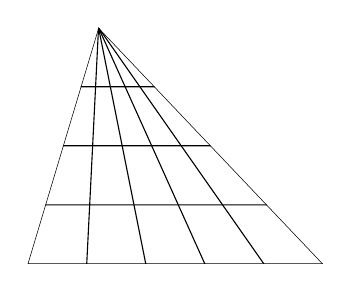
\begin{tikzpicture}[scale=0.75, font=\footnotesize, line join=round, line cap=round, >=stealth]
   \clip (0,0)--(1.2,4)--(5,0)--cycle;
	\foreach \x in {0,...,5}\draw (1.2,4)--(\x,0) (0,\x)--(5,\x);
\end{tikzpicture}
}	
	\loigiai{
		Đường thẳng nằm ngang cắt các đường nằm dọc tại $6$ điểm. Cứ $2$ điểm tùy ý này với đỉnh tam giác tạo thành một tam giác. Do đó số tam giác tạo ra là $\mathrm{C}_6^2=15$. Có $4$ đường ngang, do đó tổng số tam giác trong hình là $4\times 15=60$ tam giác.
	}

\end{ex}%!Cau!%
\begin{ex}%[Thi thử L3, THPT Lương Thế Vinh Hà Nội, 2019]%[Tô Ngọc Thy, dự án EX9]%[1D2K2-3]
	Cho đa giác đều có $20$ cạnh. Có bao nhiêu hình chữ nhật (không phải là hình vuông), có các đỉnh là đỉnh của đa giác đều đã cho?
	\choice
	{$45$}
	{$35$}
	{\True $40$}
	{$50$}
	\loigiai{
		Đa giác đều có $20$ cạnh thì sẽ có tất cả $10$ đường chéo đi qua tâm của đa giác.\\
		Một hình chữ nhật được tạo thành từ $2$ đường chéo đi qua tâm, suy ra số hình chữ nhật được tạo thành là $C_{10}^2=45$.\\
		Hình vuông được tạo thành từ $2$ đường chéo vuông góc nhau, ta có tất cả $5$ cặp đường chéo vuông góc nhau, suy ra có tất cả $5$ hình vuông.\\
		Vậy có $40$ hình chữ nhật (không phải hình vuông) được tạo thành.}
\end{ex}%!Cau!%
\begin{ex}%[Chuyên Lê Hồng Phong, Nam Định, 2019, lần 1]%[Vinh Vo 12EX9, 2019]%[1D2K2-1]
	Một hộp đựng $ 20 $ viên bi khác nhau và được đánh số từ $ 1 $ đến $ 20 $. Lấy $ 3 $ viên bi từ hộp trên rồi cộng số ghi trên đó lại. Hỏi có bao nhiêu cách lấy để kết quả thu được là một số chia hết cho $ 3 $? 
	\choice
	{$ 90 $}
	{$ 1200 $}
	{\True $ 384 $}
	{$ 1025 $}
\loigiai{
	Từ $ 20 $ số ban đầu, ta chia ra như sau 
	\begin{itemize}
		\item $ A_0 = \{ 3; 6; 9; 12; 15; 18 \} $
		\item $ A_1 = \{ 1; 4; 7; 10; 13; 16; 19 \} $
		\item $ A_2 = \{ 2; 5; 8; 11; 14; 17; 20 \} $
	\end{itemize}
	Giả sử số ghi trên viên bi khi lấy ra là $ x, y ,z $.	\\
	Tổng $ x + y + z \ \vdots \ 3 $ xảy ra trong $ 4 $ trường hợp sau
	\begin{enumerate}[TH 1.]
		\item Từ tập $  A_0 $ lấy ra $ 3  $ số  có $ \mathrm{C}^3_6 = 20 $ cách.
		\item Từ tập $  A_1 $ lấy ra $ 3  $ số có $ \mathrm{C}^3_7 = 35 $ cách.
		\item Từ tập $  A_2 $ lấy ra $ 3  $ số có $ \mathrm{C}^3_7 = 35$ cách.
		\item Mỗi tập $ A_0 $, $ A_1 $ và $ A_2 $ lấy ra $ 1 $ số có $ \mathrm{C}^1_6 \cdot \mathrm{C}^1_7 \cdot \mathrm{C}^1_7 = 294 $
	\end{enumerate}	
	Vậy có $ \mathrm{C}^3_6 + \mathrm{C}^3_7 + \mathrm{C}^3_7 + \mathrm{C}^1_6 \cdot \mathrm{C}^1_7 \cdot \mathrm{C}^1_7 =   384 $ cách.
} 
\end{ex}